%%-----------------------------------------------------------------
% Tomas James
% 4th Year Project: How good is dust emission as a tracer of star forming regions in molecular clouds?
% Cardiff University
%-----------------------------------------------------------------

%-----------------------------------------------------------------
% Start Document Preamble
%-----------------------------------------------------------------

\documentclass{report}

\usepackage[sc]{mathpazo} % Use the Palatino font
%\usepackage[T1]{fontenc} % Use 8-bit encoding that has 256 glyphs
\linespread{1.05} % Line spacing - Palatino needs more space between lines
%\usepackage{microtype} % Slightly tweak font spacing for aesthetics

\usepackage[hmarginratio=1:1,top=32mm,left=10mm,right=10mm,columnsep=15pt]{geometry} % Document margins
\usepackage[hang,small,labelfont=bf,up,textfont=it,up]{caption} % Custom captions under/above floats in tables or figures
\usepackage{booktabs} % Horizontal rules in tables
\usepackage{float} % Required for tables and figures in the multi-column environment - they need to be placed in specific locations with the [H] (e.g. \begin{table}[H])
\usepackage{hyperref} % For hyperlinks in the PDF

\usepackage{lettrine} % The lettrine is the first enlarged letter at the beginning of the text
\usepackage{paralist} % Used for the compact item environment which makes bullet points with less space between them

\usepackage{graphicx} % Used for insertion of graphics

\usepackage[english]{babel}% Recommended
\usepackage{csquotes}% Recommended

\usepackage[style=authoryear, firstinits=true, backend=biber]{biblatex}
\renewcommand*{\revsdnamepunct}{}
\renewbibmacro{in:}{} % Remove 'in' from bibliography
\DeclareNameAlias{sortname}{last-first} % Change ordering of name
\addbibresource{../refs/refs.bib}% Syntax for version >= 1.2

\usepackage{abstract} % Allows abstract customization
\renewcommand{\abstractnamefont}{\normalfont\bfseries} % Set the "Abstract" text to bold
\renewcommand{\abstracttextfont}{\normalfont\medium\itshape} % Set the abstract itself to small italic text

\usepackage{titlesec} % Allows customization of titles
\titleformat{\chapter}[display]
{\normalfont\huge\bfseries}{\chaptertitlename\ \thechapter}{20pt}{\Huge}
\titlespacing{\chapter}{0pt}{0pt}{0pt}
%\renewcommand\thesection{\Roman{section}} % Roman numerals for the sections
%\renewcommand\thesubsection{\Roman{subsection}} % Roman numerals for subsections
\titleformat{\section}[block]{\large\scshape\centering}{\thesection.}{1em}{} % Change the look of the section titles
\titleformat{\subsection}[block]{\large}{\thesubsection.}{1em}{} % Change the look of the section titles

\usepackage{listings} % Allow code to be input into appendix
\usepackage{courier}

\usepackage{verbatim}

\usepackage{wrapfig}
\usepackage{caption}
\usepackage{subcaption}

\usepackage{mhchem}
\usepackage{siunitx}

\setcounter{secnumdepth}{3}

\usepackage{fancyhdr} % Headers and footers
\pagestyle{fancy} % All pages have headers and footers
\fancyhead{} % Blank out the default header
\fancyfoot{} % Blank out the default footer
\fancyfoot[RO,LE]{\thepage} % Custom footer text
%\rhead{Student ID: 1158976}

\usepackage{dirtytalk}
\usepackage{textcomp}

\title{\vspace{-15mm}\fontsize{24pt}{10pt}\selectfont\textbf{How good is dust emission as a tracer of star forming regions in molecular clouds?}} % Article title

% Define title and author
\author{
\large
\textsc{\parbox{\linewidth}{\centering%
Tomas James\endgraf\skip
Student ID: 1158976\endgraf\bigskip}} % author name
\vspace{-5mm}
}

\date{\large\parbox{\linewidth}{\centering%
  Supervisor: Dr. P. C. Clark \endgraf\bigskip\today}}

%-----------------------------------------------------------------
% Begin Document
%-----------------------------------------------------------------

\begin{document}

\maketitle % Insert title

\thispagestyle{fancy} % All pages have headers and footers

%-----------------------------------------------------------------
% Begin Abstract
%-----------------------------------------------------------------

\begin{abstract}
A data analysis pipeline to analyse synthetic Herschel images of early star forming regions to probe the dust emission characteristics of the data was written in the Python programming language. Initially a simple scenario of a spherical molecular cloud was simulated using RADMC-3D \parencite{RADMC-3D}, with bespoke input files generated using the Python programming language. This simulation was performed across the 3 SPIRE \parencite{SPIRE} wavebands centered on 250 $\mu m$, 350 $\mu m$ and 500 $\mu m$ as well as the 3 PACS \parencite{PACS} wavebands centered on 72 $\mu m$, 103 $\mu m$ and 167 $\mu m$. This data was then `degraded` by accounting for the instrument's transmission curve to better simulate an object observed by Herschel. This data was then subsequently analysed by plotting Spectral Energy Distributions (SEDs) on a pixel by pixel basis to recover the column density $N$ and temperature $T$ at each pixel. The goodness-of-fit was assessed using a $\chi^{2}$ test. 2-dimensional maps of these regions was then constructed and the recovered values of $N$ and $T$ compared to the initial input values of density and temperature. Finally this machinery was applied to data from the SPH simulation Arepo to emulate real Herschel data.
\end{abstract}

%-----------------------------------------------------------------
% Begin Contents
%-----------------------------------------------------------------

\tableofcontents % Insert table of contents
\pagebreak % Adds page break after contents

%-----------------------------------------------------------------
% Introduction
%-----------------------------------------------------------------

\chapter{Introduction}

\section{Molecular clouds}
A molecular cloud is a dense region of the Interstellar Medium (ISM), composed primarily of molecular Hydrogren ($H_{2}$) at temperatures $<$ 20 $K$ \parencite{dustopacity}. Despite the cloud being primarily a gas of $H_{2}$, a small (by mass) dust component is also present. This dust mass component is approximately 1\% the gas mass according to \textcite{noise}, however despite this minimal presense dust remains a crucial component in the evolution of the cloud and the subsequent star forming process.

\begin{wrapfigure}{l}{0.5\textwidth}
  \begin{center}
    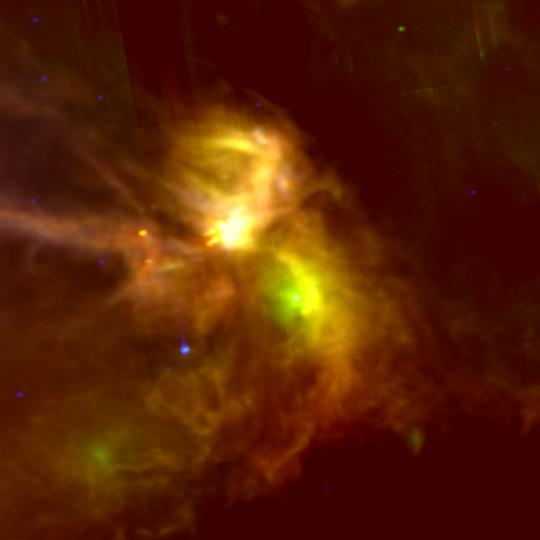
\includegraphics[width=0.4\textwidth]{../img/rho.jpg}
    \caption[An IRAS image showing the Rho Opiuchi cloud complex \parencite{rho}.]{An IRAS image showing the Rho Opiuchi cloud complex \parencite{rho}.}
  \end{center}
\end{wrapfigure} \label{fig:rho}

Figure \ref{fig:rho} shows the Rho Ophiuchi cloud complex as imaged by the Infra-red Astronomical Satellite (IRAS). Rho Opiuchi is the nearest active star forming molecular cloud complex to the Milky Way\footnote{\textcite{rho-dist} estimates the range of distances as being between 125pc-165pc - a range of almost 40\%.}. As a result of this, Rho Ophiuchi provides an unprecedented oppurtunity to study the sites of early star formation at high resolution. This is in spite of the large uncertainty in estimates of the distance to Rho Ophiuchi \parencite{rho-dist}.

Much like the ISM, molecular clouds are composed of gas and cosmic dust, however a molecular cloud differs from the ISM in that significantly greater densities are found within a molecular cloud than that of the ISM. The dust density in a molecular cloud is thought to be around $10^{5}\,g\,cm^{-3}$, whilst the dust density in the surrounding ISM is thought to be around $10^{2}\,g\,cm^{-3}$.

The molecular cloud is also colder than the surrounding ISM: the temperature is approximately 15 $K$ in the ISM whilst the temperature in the molecular cloud is approximately 10 $K$. The warmer ISM bathes the cooler cloud, resulting in a temperature gradient; the ISM heats the cloud from the outside in, resulting in a temperature that increases with distance from the centre of the cloud.

Figure \ref{fig:rho} illustrates the intense infra-red emission within molecular clouds owing to the active star forming occurring within them. It also illustrates the turbulence and chaos within the cloud, with both filamentary structure and (potentially) magnetic fields running through the cloud itself. These filaments are regions of higher density, and as \textcite{evo-mol} states \say{One fundamental characteristic of molecular clouds is that they are not, as has sometimes been assumed, isolated ‘billiard balls’ moving about independently in space, but instead are just dense condensations in more widely distributed, mostly atomic gas. Although molecular clouds may often appear to have sharp boundaries, these boundaries do not represent the edge of the matter distribution but just rapid transitions from the molecular gas to the surrounding atomic gas, which is distributed in extended envelopes that typically have comparable mass (Blitz 1988, 1991)}. These filaments act as preferential sites for star formation \parencite{filaments}.

These star forming regions within molecular clouds originate from locations of gravitational instability that lead to subsequent collapse \parencite{jeans}. A stable cloud (or portion of a cloud) is in hydrostatic equilibrium, such that the force due to gravity is balanced by the force due to gaseous pressure from the gas within the cloud. This equilibrium state can also be regarded as a virialised state such that $2K+U=0$, where $K$ is the total kinetic energy of the system and $U$ is the total potential energy of the system. The cloud begins to collapse when the gravitational force is greater than the force due to the hydrostatic pressure. This collapse continues unimpinged until such a time that another opposing force can halt the collapse. The initial collapse is triggered when a region within the molecular cloud has a mass that exceedes the Jeans' mass given by Equation \ref{eq:jeans} \parencite{lecture}. This is known as the Jeans Criterion.

\begin{equation}\label{eq:jeans}
  M_{J} = \Bigg( \frac{5kT}{GM} \Bigg )^\frac{3}{2} \Bigg( \frac{3}{4\pi\rho} \Bigg )^\frac{1}{2}
\end{equation}

Within Equation \ref{eq:jeans}, $k$ is the Stefan-Boltzmann constant, $T$ is the temperature of the region, $G$ is the Universal Gravitational Constant, $M$ is the mass of Hydrogen in the region and $\rho$ is the density of the region prior to collapse. The collapse of an $M_{J}$ mass region occurs according to the free-fall time, $t_{ff}$ described in Equation \ref{eq:tff} \parencite{krumholz}.

\begin{equation}\label{eq:tff}
  t_{ff} = \sqrt{\frac{3\pi}{32G\rho}}
\end{equation}

Variables within Equation \ref{eq:tff} are as they were defined in Equation \ref{eq:jeans}.

Interestingly the onset of collapse is also the onset of gravitational binding. According to \textcite{bound}, the majority of a molecular cloud remains gravitationally unbound, further reinforcing the idea stated in \textcite{evo-mol} that molecular clouds are diffuse, transiest structures.

\begin{comment}
  \section{Star Formation}
  The star forming process is one of the most important processes in the cosmos, as star formation (and the subsequent evolution of the star) poses an unequivocal factor driving the evolution of the Universe forward.

  Stars are essentially chemical foundaries, acting as the primary source of elements heavier than \ce{^{2}He} in the Universe. The production of \ce{^{1}H} is thought to have occured approximately 380,0000 years after the Big Bang \parencite{peebles}, when the primordial quark-gluon plasma had cooled sufficiently to allow protons and neutrons (hereafter $p$ and $n$) to bind and form atoms. \ce{^{2}He}, according to \textcite{bbc}, also formed at this time however the fundamental particles required to form elements were produced within the first few seconds after the Big Bang. Whilst further production of \ce{^{2}He} can occur via the first fusion process, the proton-proton (pp) reaction described by Equation \ref{ppchain} \parencite{synthesis} is the primary source of \ce{^{2}He} in stars. This is in stark contrast to \ce{^{1}H}, which cannot be produced via a fusion process.

  \begin{equation} \label{ppchain}
    \ce{^{1}{H} + ^{1}{H} -> ^{2}{He} + e^{+} + v_{e} + 0.42 MeV}
  \end{equation}

  Despite the lack of \ce{^{1}H} production, \ce{^{1}H} is still the most abundant element in the Universe, amounting to roughly 72\% by mass according to \textcite{abundance}. This relative prevalence of \ce{^{1}H} is known as a direct result of observations of the $21cm$ line \parencite{21cm}. The $21cm$ line originates from the hyperfine splitting that occurs when the only electron in \ce{^{1}H} in the $1s$ orbital spin flips to become antiparellel with the spin of the nucleus. This produces the characteristic photon emission at $\lambda=21cm$. This transition corresponds to a temperature of $T~0.014 K$ according to Wien's displacement law $\lambda_{max}=0.0029/T$, meaning the excitation can occur almost anywhere in the Universe.

  \subsection{Fusion}
  The fusion process occuring within stars adapts and evolves with the star itself. After the star has undergone its initial fusion process described in Equation \ref{ppchain}, it begins to cool.

  \ce{^{56}Fe} cannot be fused to create any heavier elements as this fusion requires more energy to fuse than the fusion would produce, thus acting as a net loss of energy. As a direct result of this, fusion stops within a star at \ce{^{56}Fe}.
\end{comment}

\section{Dust emission}
Dust is a relatively small fraction of the total ISM mass, estimated as being only 1\% according to \textcite{noise}. Whilst the dust mass accounts for such a small mass component, it still presents an important role in forming stars. The sources of flux embedded deep within the cloud radiate across a wide range of wavelengths, however the dust surrounding the source has the effect of absorbing and then re-radiating photons at a different wavelength. As such, these sources of flux (be they prestellar cores, protostars or pre-main sequence stars) are occluded by the dust enveloping them.

Dust radiates as a modified black body approximated by Equation \ref{eq:mbb} \parencite{noise}.

\begin{equation} \label{eq:mbb}
  S_{\nu} = N \Omega \kappa_{0} \Big(\frac{\nu}{\nu_{0}}\Big)^{\beta} B_{\nu}(T)
\end{equation}

In Equation \ref{eq:mbb} $S_{\nu}$ is the flux density, $N$ is the column density, $\Omega$ is the solid angle subtended by the beam, $\kappa_{0}$ is a reference dust opacity, $\nu$ is the frequency of the image, $\nu_{0}$ is a reference frequency at which the reference opacity $\kappa_{0}$ was evaluated at, $\beta$ is the dust spectral index and $B_{\nu}(T)$ is the frequency dependent Planck function. In terms of intensity:

\begin{equation} \label{eq:mbb-int}
  I_{\nu} = \frac{N}{R_{dust-gas}} \mu m_{p} \kappa_{0} \Big(\frac{\nu}{\nu_{0}}\Big)^{\beta} B_{\nu}(T)
\end{equation}

All variables in Equation \ref{eq:mbb-int} are as defined in Equation \ref{eq:mbb}, with the addition of $R_{dust-gas}$. $R_{dust-gas}$ is the dust-to-gas ratio, here approximated as being $\frac{1}{100}$. Throughout this project, dust emission was quantified in terms of intensity rather than flux density, as intensity is independent of distance to the source of emission.

Dust properties such as the spectral index $\beta$ and temperature $T$ clearly have an effect on dust emission according to Equations \ref{eq:mbb} and \ref{eq:mbb-int}. These parameters therefore effect the ability to detect radiation from within a molecular cloud.

\section{Herchel Space Observatory}
The Herschel Space Observatory was an ESA mission launched in 2009 with the primary objective of imaging cold regions of the Universe \parencite{herschel} and \parencite{fact}. Herschel had a number of objectives. As \textcite{fact} states, these objectives included ``targeted observations of star formation and both young and old stars, to reveal the physical and chemical processes in the early and later phases of a star’s life.'' To achieve this, Herschel was launched with 3 different instruments onboard: Photodetector Array Camera and Spectrometer: PACS \parencite{PACS}, Spectral and Photometric Imaging Receiver: SPIRE \parencite{SPIRE} and Heterodyne Instrument for the Far Infrared: HiFi \parencite{HiFi}. One of these instruments, SPIRE, was designed to probe the sites of early star formation deep within molecular clouds. This was achieved by imaging solely in the infra-red and sub-mm regimes. Herschel itself, across all instruments and functional modes, is sensitive to a range of wavelengths quoted by \textcite{herschel} as $~55-672 \micro\meter$. SPIRE itself had an photometry wavelength range $~200-670 \micro\meter$ whilst PACS was sensitive to a photometry wavelength range $~60-210 \micro\meter$. This therefore produces effectively continuous coverage of the wavelength range $~60-670$\footnote{Further coverage is achieved down to $55 \micro\meter$ using HiFi however this is only achievable for spectroscopic applications.}

In order to achieve the effective wavelength range described above, both SPIRE and PACS detectors required extensive cooling to a temperature of $0.3 K$ via $^{3}{He}$ sorption coolers \parencite{herschel}. Again according to \textcite{herschel} the image focal plane required cooling to $1.7 K$, again achieved using 2160 litres of Helium cryogen. To minimise any thermal radiation from the observatory itself, the spacecraft was radiatively cooled to a temperature of $85 K$ \parencite{herschel}. These temperatures allowed effective detection (via a bolometric detector in the case of SPIRE and a photometer in the case of PACS) of infra-red and sub-mm photons. 

\section{RADMC-3D} \label{radmc}
RADMC-3D is a 3-dimensional Monte-Carlo radiative transfer and ray tracing code developed by Cornelis Dullemond and written in Fortran 90 for radiative transfer and emission astrophysics in dusty environments \parencite{RADMC-3D}.

RADMC-3D is able to compute dust emission intensity as well as Spectral Energy Distributions (SED) and spectra for a number of different continua. This project focussed only on dust continuum, neglecting gas. The dust emission intensity can be computed using 2 different methods: the thermal Monte-Carlo simulation, or an image ray trace. All computations require input files for RADMC-3D to read and use in its simulations. RADMC-3D \textquotesingle s Python port, \texttt{radmc3dPy} \parencite{radmc3dPy}, is able to write these input files, however for this project a custom script was written such that file creation was independent of \texttt{radmc3dPy}.

\subsection{\texttt{radmc3dPy}}
Whilst RADMC-3D is written in Fortran 90, a Python ‘wrapper’, \texttt{radmc3dPy} allows Python to handle RADMC-3D objects.

\subsection{Input files} \label{inp}
As stated in Section \ref{radmc}, RADMC-3D requires a number of user defined input files in order to operate. These input files act as parameter spaces, defining boundary conditions along with step sizes for each given input files. Figure \ref{radmc3d-workflow} shows a workflow of RADMC-3D's operation, including all files required in order to operate.

\begin{figure}[h]
  \centering
  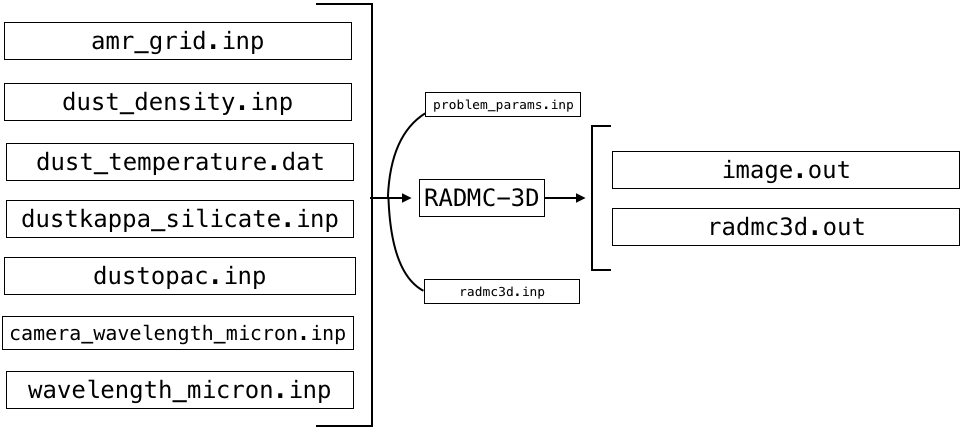
\includegraphics[scale=0.4]{../img/radmc3d-workflow}
  \caption[A schematic representation of the RADMC-3D workflow.]{A schematic representation of the RADMC-3D workflow.}
  \label{fig:radmc3d-workflow}
\end{figure}

As Figure \ref{fig:radmc3d-workflow} illustrates, all input files to RADMC-3D have extension \texttt{.inp} whilst all output files have extension \texttt{.out}. Any intermediate files, such as those directly calculated by RADMC-3D, have extension \texttt{.dat}. \textit{Most} input files' initial lines - the header information - contain quantitative information regarding the number of pixels/cells in the file, the pixel/cell width along with other identifiers that inform RADMC-3D whether to look for binary files, the number of dust species being considered and so on.

\texttt{amr\_grid.inp} is the file used in order to create a spatial domain within the model. It does this by defining the start and end points of pixels in 3 dimensions: x, y and z. These definitions produce pixels, each of fixed width defined by the distance between pixel start and end points. RADMC-3D also has the ability to perform Adaptive Mesh Refinement, such that regions of interest can be split into more pixels (and have a smaller pixel width and therefore simulated higher resolutions) than, for example, regions of the ISM that do not require a higher resolution. Any further files that setup physical quantities draw directly from the structure of \texttt{amr\_grid.inp}. They essentially \textquotesingle insert \textquotesingle a value of a physical quantity into each cell, therefore producing another parameter space. This structure is illustrated in Figure \ref{fig:amr_grid_structure}.

\begin{wrapfigure}{r}{0.5\textwidth}
  \centering
  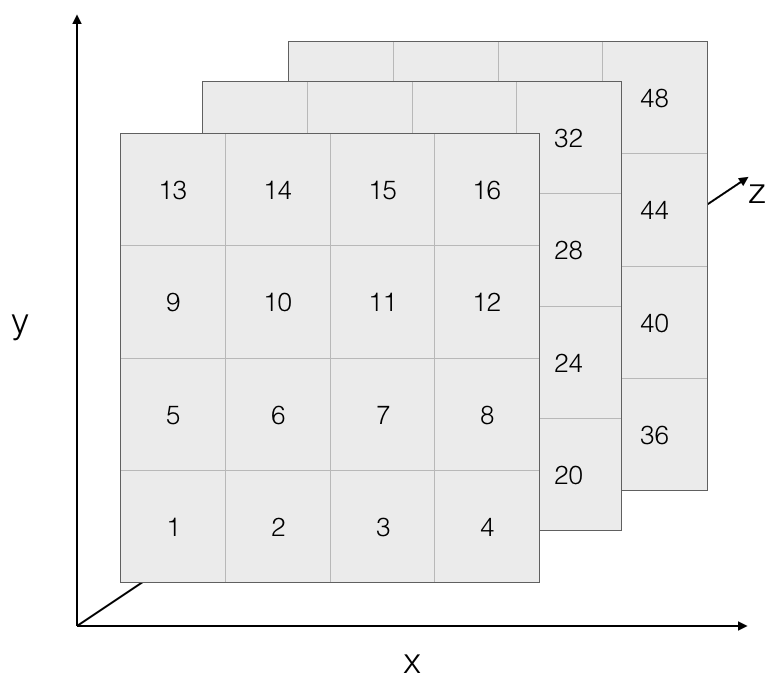
\includegraphics[scale=0.3]{../img/amr_grid_structure}
  \caption[A pictorial representation of the structure of \texttt{amr\_grid.inp} for a 4x4x3 grid. The index of a cell, denoted by the number contained within it, is the position of that cell in \texttt{amr\_grid.inp}.]{A pictorial representation of the structure of \texttt{amr\_grid.inp} for a 4x4x3 grid. The index of a cell, denoted by the number contained within it, is the position of that cell in \texttt{amr\_grid.inp}.}
\end{wrapfigure}\label{fig:amr_grid_structure}

The index of each cell in Figure \ref{fig:amr_grid_structure} is that cell's position in \texttt{amr\_grid.inp}. For example,

\texttt{dust\_density.inp} is the file that gives RADMC-3D its density information. It has the same structure as \texttt{amr\_grid.inp}, however in place of the start and end pixel points that are found in \texttt{amr\_grid.inp}, \texttt{dust\_density.inp} defines the dust density (in $cgs$ units) at each pixel. This therefore creates a density parameter space with which to work from. Similarly, \texttt{dust\_temperature.dat} draws upon the same idea, however instead of defining dust densities, \texttt{dust\_temperature.dat} defines the dust temperature (in $K$) at each pixel point. These 3 files therefore create 3 parameter spaces: spatial, density and temperature.

Another crucial file is the \texttt{wavelength\_micron.inp} file. This input file defines the wavelengths over which RADMC-3D should compute. By default, \texttt{wavelength\_micron.inp} runs from $\SI{0.1}{\micro\meter}$ to $\SI{1000}{\micro\meter}$ with $150$ points. Dust emission intensity can then be determined at any wavelength between these two bounds. In reality however, computing dust emission intensity over such a wide wavelength range is not always necessary (or practical). RADMc-3D thus allows the user to define a \texttt{camera\_wavelength\_micron.inp} file. This file is designed to constrict the range of wavelengths over which RADMC-3D computes, thus emulating the wavelengths available to a given telescope or filter. In this project \texttt{camera\_wavelength\_micron.inp} was used in order to allow RADMC-3D to compute dust emission intensity in wavelength bands corresponding to those found on both SPIRE \parencite{SPIRE} and PACS \parencite{PACS}.

\subsection{Thermal Monte-Carlo dust emission} \ref{mctherm}
The thermal Monte-Carlo simulation is able to compute dust temperatures – using the technique described in \textcite{b&w} – from user-defined dust densities, providing a source of flux (and therefore photons) exists. This source of flux can either be through a star in the image space or an Interstellar Radiation Field. The process used to compute the dust temperature, according to \textcite{manual}, is as follows. The total luminosity of the source is first split into $nphot$ photon packets. The code then proceeds to \textquotesingle fire \textquotesingle photons out from the flux source into the image space. These photons can then either scatter off of dust grains or be absorbed by one, thus immediately being re-emitted at a different wavelength and direction as defined in \textcite{b&w}. Under scattering/re-emission the photon will travel through the image space as defined in \texttt{amr\_grid.inp} - see Section \ref{inp} - entering different adjoining pixels as it does so. This increases the temperature of that pixel, again according to \textcite{b&w}. This process of \textquotesingle ping-ponging \textquotesingle throughout the image space is continued until the photon packet leaves the image space. At this point, a new photon packet is \textquotesingle fired \textquotesingle and the process is repeated using the previously determined dust temperatures until no further photon packets remain. The dust temperature at this point is therefore the solution.

Naturally the more pixels an image space comprises then the longer the simulation takes to compute owing to the large number of pixels and therefore collisions encountered. Likewise the greater the dust density at a given point the longer the simulation takes to run owing to a similar effect. Normally, RADMC-3D would write the calculated dust temperatures to \texttt{dust\_temperature.dat} however as the thermal Monte-Carlo simulation was not used in this project, RADMC-3D was supplied with idealised dust temperatures in the form of a pre-determined \texttt{dust\_temperature.dat} file.

\subsection{Ray tracing dust emission} \ref{rt_des}
Conversely the image ray trace reads in both user-defined dust temperatures and dust densities, thus bypassing the computation of the dust temperatures as would have been the case in the thermal Monte-Carlo simulation. Again, according to \textcite{manual}, the ray-trace follows, by default, a first-order integration where the source function, $S = j_{\nu}/\alpha$ and opacity (and therefore extinction $\alpha$) are constant across the ray. This is described by Equation \ref{raytrace}.

\begin{equation}
  I_{result} = I_{start}e^{-\tau}+(1+e^{-\tau})S
\end{equation}\ref{raytrace}

$I_{result}$ is the dust emission intensity of the cell, $I_{start}$ is the dust emission intensity of the cell prior to the ray entering it and $\tau$ is the optical depth along the path of the ray through the cell. The optical depth $\tau$ is defined as $\tau = \alpha s$ where $\alpha$ is as defined earlier and $s$ is the distance the ray travels through the cell. The option to perform second-order integration is also made possible by varying the source function $S$ and extinction across the ray. Specifically $S$ and $\alpha$ are fixed at the ingress and egress points of the ray. These points act as boundary conditions such that the variation in $S$ amd $\alpha$ can then be linearly interpolated across the path of the ray through the cell.

The result, however, is the same in both Thermal Monte-Carlo simulation and ray-trace: an \texttt{image.out} file that contains the dust emission intensity at each cell in the image plane. RADMc-3D is also capable of accounting for scattering of photons off of dust grains however this project focussed solely upon absorption and re-emission only.

\chapter{Methodology}

\section{Model setup}

\subsection{Example scripts}
RADMC-3D includes a number of basic example scripts to familiarise the user with the software's operation and capabilities. As a result, they provide an excellent introductory exercise to using RADMC-3D. Examples of 1D and 2D thermal Monte-Carlo simulations were run in this regard, generating Figures \ref{fig:1d} and \ref{fig:2d}.

\begin{figure}[!htb]
\minipage{0.48\textwidth}
  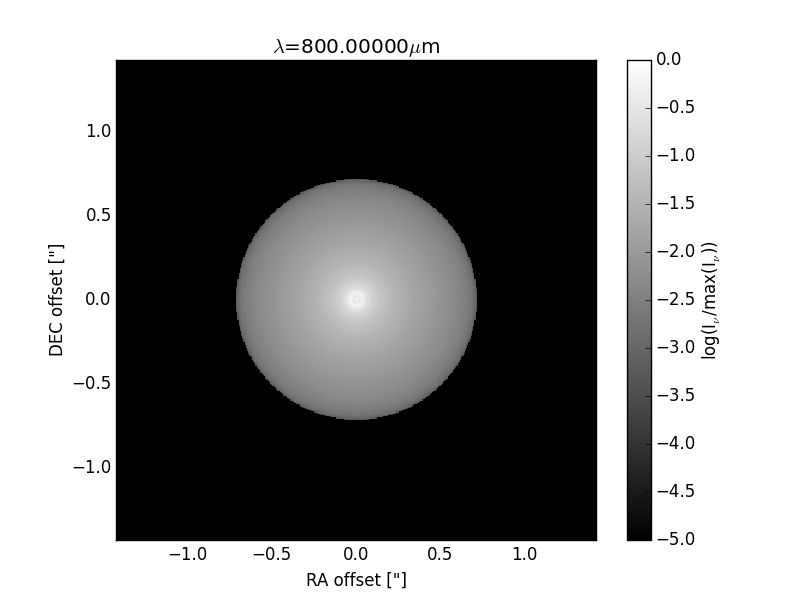
\includegraphics[width=\linewidth]{../img/1d}
  \caption{The RADMC-3D output for dust emission intensity computed using thermal Monte-Carlo simulation in 1D.}\label{fig:1d}
\endminipage\hfill
\minipage{0.48\textwidth}
  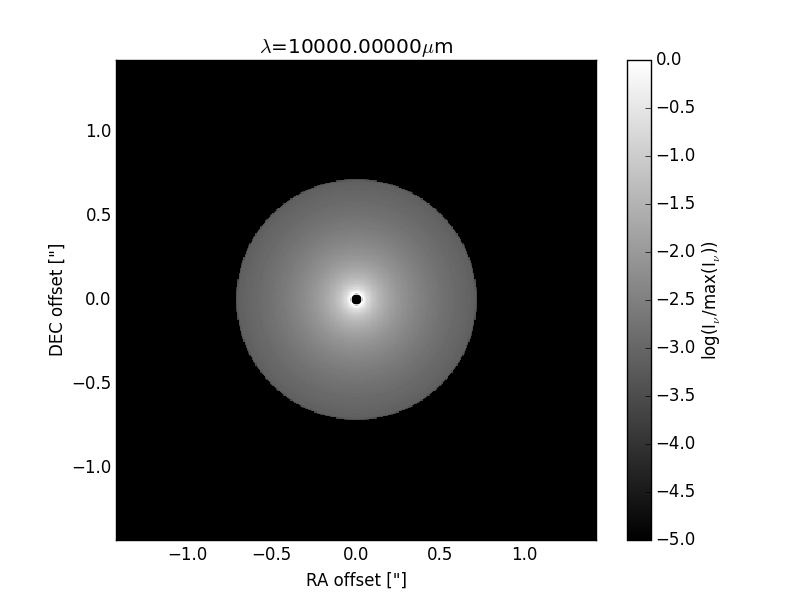
\includegraphics[width=\linewidth]{../img/2d}
  \caption{The RADMC-3D output for dust emission intensity computed using thermal Monte-Carlo simulation in 2D.}\label{fig:2d}
\endminipage
\end{figure}

In order to begin operation, RADMC-3D's example scripts were analysed and run. The examples were used to understand how RADMC-3D generated the input files required (and as discussed in Section \ref{inp}) as well as how the code used them and for what purpose. These examples were basic, consisting of both 1D and 2D sphere projections with user defined stars at their centres.

These examples ran thermal Monte-Carlo simulations. The first stage in this computation after writing the input files from the user inputs was to build dust temperatures. This was achieved using the process described in Section \ref{mctherm}. Once dust temperatures had been computed, RADMC-3D then performed a ray-trace in order to build the dust emission intensity. This was again achieved using the method described in Section \ref{rt_des}.

\subsection{Modelling a cloud}
To begin building 3D models outside of the example scripts, specific input files needed to be created. As stated, a custom Python script was written to handle this file creation. Traditionally, \texttt{radmc3dPy} would handle file creation at the model setup phase, however given that RADMC-3D is designed to be run from the command line it was determined that reducing the number of dependencies would allow greater compatibility with different machines. This is critical if the code was to be run on a machine that may not have \texttt{radmc3dPy} installed, such as a supercomputer for larger computations. This also resulted in some of \texttt{radmc3dPy\textquotesingle}s model setup commands being made redundant. For example, \texttt{radmc3dPy.setup.problemSetupDust} sets up the model using input parameters that are parsed to a model file. This phase was handled solely by \texttt{datafilegen.py}, so this command was redundant. Instead, required parameters such as the number of pixels in each dimension was given to RADMC-3D when calling it from the command line using \texttt{os.system(radmc3d image loadlambda)}. Again, the image ray-trace could be initiated through Python via the \texttt{os.system(radmc3d image)} command. The \texttt{loadlambda} keyword informs RADMC-3D that it should use the \texttt{camera\_wavelength\_micron.inp} module.

RADMC-3D then performs its raytrace and outputs the computed intensities to an \texttt{image.out} file. This image is a 2D image with image dimensions in the x-y plane corresponding to the initial x and y image dimensions supplied to RADMC-3D. This file contains the dust emission intensity values at each pixel within that plane. This intensity is, however, an idealised intensity that does not account for any ineffeciences. It was assumed that the source is imaged in the absence of any occluding material, thus exctinction was neglected. It was necessary however in order to simulate data as imaged by Herschel to account for the frequency dependent transmission of Herschel's filters.

\subsection{Simulating Herschel}
No telescope or observatory can produce perfect images or data; components within the telescope, the observatory or the surroundings all degrade the data quality. Refraction at the telescope aperture  Not all photons that fall on a filter are transmitted owing to reflection off of the filter itself. This is frequency dependent and thus produces a ``transmission curve''.

\section{Appendix}
All code was version controlled using GitHub and stored in a private repository throughout development. The repository containing all code can be found at \href{http://www.github.com/tomasjames/ZiggyStarDust}{http://www.github.com/tomasjames/ZiggyStarDust}.

%-----------------------------------------------------------------
% Bibliography
%-----------------------------------------------------------------

\printbibliography

%\nocite{*}
%\printbibliography

%-----------------------------------------------------------------
% Appendix
%-----------------------------------------------------------------

\end{document}
